
 \begin{figure}[h!]
 	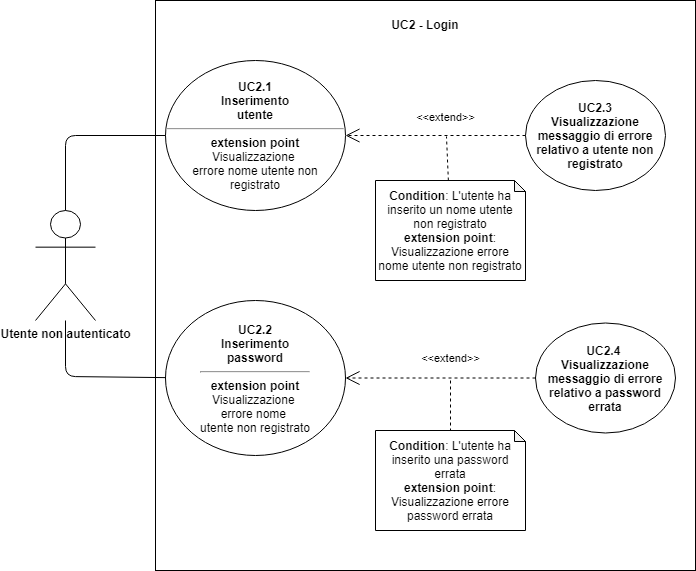
\includegraphics[width=17cm]{images/UC2.png}
 	\caption{Diagramma UC2}
 \end{figure}
\subsection{UC2 - Login}
\begin{itemize}
	\item \textbf{Attori Primari:} utente non autenticato;
	\item \textbf{Descrizione:} l'utente tenta di autenticarsi usando le sue credenziali;
	\item \textbf{Scenario principale:} l'utente non è ancora autenticato nella piattaforma ed esegue il login;
	\item \textbf{Pre-condizione:} l'utente non è autenticato nella piattaforma;
	\item \textbf{Post-condizione:} l'utente si autentica con successo, l'utente viene identificato dal sistema nel ruolo di amministratore o operatore. A seconda del ruolo vengono rese disponibili diverse funzionalità.
\end{itemize}

\subsubsection{UC2.1 Inserimento nome utente}
\begin{itemize}
	\item \textbf{Attori Primari:} utente non autenticato;
	\item \textbf{Descrizione:} al fine di potersi autenticare, l'utente è tenuto ad inserire il suo nome utente, campo obbligatorio;
	\item \textbf{Scenario principale:} l'utente inserisce il suo nome utente;
	\item \textbf{Pre-condizione:} il sistema ha reso disponibile il campo per l'inserimento del nome utente;
	\item \textbf{Post-condizione:} l'utente compila il campo con il proprio nome utente.
\end{itemize}	

\subsubsection{UC2.2 Inserimento password}
\begin{itemize}
	\item \textbf{Attori Primari:} utente non autenticato;
	\item \textbf{Descrizione:} al fine di potersi autenticare, l'utente è tenuto ad inserire la sua password, campo obbligatorio;
	\item \textbf{Scenario principale:} l'utente inserisce la sua password;
	\item \textbf{Pre-condizione:} il sistema ha reso disponibile il campo per l'inserimento della password;
	\item \textbf{Post-condizione:} l'utente compila il campo con la propria password.
\end{itemize}	

\subsubsection{UC2.3 Visualizzazione messaggio di errore relativo a utente non registrato}
\begin{itemize}
	\item \textbf{Attori Primari:} utente non autenticato;
	\item \textbf{Descrizione:} l'utente visualizza un messaggio d'errore dovuto al fatto che ha tentato il login con un nome utente non registrato;
	\item \textbf{Scenario principale:} l'utente cerca di fare il login senza essere stato registrato;
	\item \textbf{Pre-condizione:} l'utente cerca di autenticarsi nella piattaforma;
	\item \textbf{Post-condizione:} viene visualizzato un messaggio d'errore per notificare l'utente che un amministratore non ha registrato il suo nome utente nel sistema.
\end{itemize}

\subsubsection{UC2.4 Visualizzazione messaggio di errore relativo a password errata}
\begin{itemize}
	\item \textbf{Attori Primari:} utente non autenticato;
	\item \textbf{Descrizione:} l'utente visualizza un messaggio d'errore dovuto al fatto che ha tentato il login con una password errata;
	\item \textbf{Scenario principale:} l'utente cerca di fare il login con una password sbagliata;
	\item \textbf{Pre-condizione:} l'utente cerca di autenticarsi nella piattaforma;
	\item \textbf{Post-condizione:} viene visualizzato un messaggio d'errore per notificare l'utente ha inserito una password sbagliata.
\end{itemize}



